% JBJI thesis open-source template.
% By JBJI 2022 grade students.(2026/4/5)
% 改编自原暨南大学论文latex模板（2021/06/21）

\documentclass[master]{jnuthss}

\usepackage{xcolor}
\usepackage{booktabs}
\usepackage{graphicx}
\usepackage{amsmath}
\usepackage{amssymb}
\usepackage{microtype}
\usepackage{enumitem}
\usepackage{float}
\usepackage{subcaption}
\usepackage{multirow}
\usepackage{array}
\usepackage{longtable}
\usepackage{tabularx}
\usepackage{siunitx}
\usepackage{caption}
\usepackage{cleveref}
\usepackage{tikz}
\usepackage{pgfplots}
\usepackage[section]{placeins}
\pgfplotsset{compat=1.18}
\usetikzlibrary{shapes.geometric, arrows.meta, positioning, fit, calc, backgrounds}

\etitle{Sample JBJI Undergraduate Thesis Title}
\etitlelinea{Sample JBJI Undergraduate Thesis}
\etitlelineb{Title in English}
\ctitle{中文论文题目示例}
\author{Student Name}
\cauthor{学生姓名}
\studentid{2022000000}
\emajor{Programme Name}
\cmajor{专业名称}
\esupervisor{Supervisor Name}
\csupervisor{指导教师姓名}
\college{暨南大学伯明翰大学联合学院}
\department{}
\edate{dd/mm/yyyy}
\cdate{YYYY年MM月DD日}

\graphicspath{{figures/}}

\begin{document}

\maketitle{}
\makestatement{}
\frontmatter

\thispagestyle{plain}

{
  \centering\jnuthssAbstractTitleFont Sample JBJI Undergraduate Thesis Title\par
  \vspace{\jnuthssAbstractTitleInnerGap}
}

\vspace{\jnuthssAbstractBodyTopSpace}

{\jnuthssAbstractBodyStyle\noindent\textbf{Abstract:}
This is a neutral abstract placeholder for the public JBJI thesis template. It
is intentionally generic and can be replaced directly by the student's own
research summary. The abstract should briefly state the research problem, the
method, the main findings, and the contribution. In normal use, the abstract is
expected to be about 300 words and followed by 3--8 keywords.
}

\vspace{\jnuthssAbstractKeywordsTopSpace}

{\jnuthssAbstractBodyStyle\noindent\textbf{Keywords:} keyword one; keyword two; keyword three; keyword four}

\thispagestyle{plain}

{
  \centering\jnuthssAbstractTitleFont 中文论文题目示例\par
  \vspace{\jnuthssAbstractTitleInnerGap}
}

\vspace{\jnuthssAbstractBodyTopSpace}
\vspace{\jnuthssAbstractCNBodyExtraTopSpace}

{\jnuthssAbstractBodyStyle\noindent\textbf{摘要：}
这里是公开版 JBJI 论文模板的中文摘要占位内容。当前文本仅用于演示摘要页的版式、
行距和关键词格式，不包含任何私有论文内容。正式使用时，可直接替换为自己的研究
背景、方法、主要结果与贡献概述。
}

\vspace{\jnuthssAbstractKeywordsTopSpace}

{\jnuthssAbstractBodyStyle\noindent\textbf{关键词：}模板；论文格式；占位内容；JBJI}

\jnuthssmaketableofcontents

\mainmatter

% Placeholder chapter for the JBJI thesis open-source template.
% Public template version with neutral placeholder content.

\chapter{Introduction}

The main text should be typed in Font Times New Roman, Size 12. No indention is needed for the first paragraph. One Tab of indention is used for the rest paragraphs. Line spacing should be 1.5 times. Also there should be no empty lines between paragraphs.

If any information or opinion is someone else's copyright, the author should be credited in the main text, for example \cite{smith2001taxation}. If the cited source is an organization rather than a specific person, it should still be cited in the same author-year format, for example \cite{worldbank2004income}. For Chinese names, the in-text citation should use the surname or family name only, as shown in \cite{liu2005income}. At the end of the main text, the references page should list the corresponding bibliographic details automatically.

% Placeholder chapter for the JBJI thesis open-source template.
% Public template version with neutral placeholder content.

\chapter{Theoretical Background}

\section{Definitions}

If any information or opinion is someone else's copy right, you should give credit to the author (Smith, 2001). And in the end of the main text, a list of reference should include the details of this citation. Please do not use footnotes, or subscripts to label references. If the information you cited is not provided by a specific person, but an organization, the reference should still be treated the same way (World Bank, 2004). The name of organization will replace the last name of author. For Chinese names, please list the surname or family name of the author only (Liu, 2005). And at the end of text, where you list all of your references, the author's full name should be given.

\section{Theories}

If you have charts, tables for illustration, please make sure that they must be self explaining (readers can understand them without reading the text). Each table should have table number, table title, and source of information. Each illustration (chart) should also have figure number, figure title, and source of data. All tables must be numbered numerically, so must the figures. Table title is on top of the table. Figure title is at the bottom of the figure. Table and figure are in separate order.

\begin{table}[htbp]
    \centering
    \small
    \caption{Theoretical Evolution of Political and Economic Integration}
    \label{tab:integration}
    \begin{tabularx}{0.9\textwidth}{@{}lXX@{}}
        \toprule
        \textbf{Stage} & \textbf{Political Feature} & \textbf{Economic Feature} \\
        \midrule
        Early stage & Policy coordination begins. & Initial resource circulation appears. \\
        Middle stage & Institutional links become clearer. & Cross-regional cooperation expands. \\
        Advanced stage & Governance mechanisms become stable. & Integration becomes more systematic. \\
        \bottomrule
    \end{tabularx}
    \caption*{}
\end{table}

\begin{figure}[htbp]
    \centering
    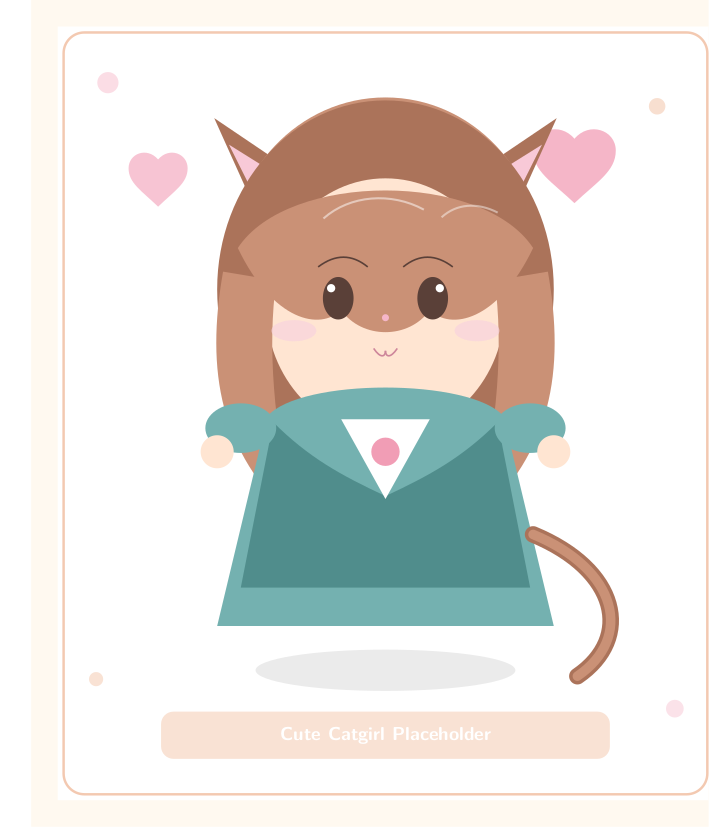
\includegraphics[width=0.58\textwidth]{catgirl-placeholder.png}
    \caption{Cute catgirl placeholder illustration.}
    \label{fig:catgirl}
    \caption*{}
\end{figure}
\FloatBarrier

% Placeholder chapter for the JBJI thesis open-source template.
% Public template version with neutral placeholder content.

\chapter{The Case Studies}

\section{Case Study One}

\subsection{The Problem Presented}

Placeholder text.

\subsection{The Analysis of the Problem}

Placeholder text.

\subsection{The Solutions Suggested}

Placeholder text.

\section{Case Study Two}

\subsection{The Problem Presented}

Placeholder text.

\subsection{The Analysis of the Problem}

Placeholder text.

\subsection{The Solutions Suggested}

Placeholder text.

% Placeholder chapter for the JBJI thesis open-source template.
% Public template version with neutral placeholder content.

\chapter{Conclusion}

The conclusion should be a summary of the problems identified and analyzed, the solutions suggested and comments by the author.

\chapter{Official-format Reminder}

The table of content should include all parts of the paper, such as introduction, conclusion, acknowledgement, appendix, and references. The page number of these sections should be listed as well.

The sample structure in the official format can be kept as a neutral placeholder outline:

\begin{enumerate}[label=\arabic*.]
    \item Introduction
    \item Literature review on financial integration
    \item The theoretical basis of financial integration
    \item Analyzes the current situation of financial integration in Guangdong, Hong Kong and Macao
    \item Empirical analysis of the financial integration of Guangdong, Hong Kong and Macao
    \item Conclusion
\end{enumerate}




\backmatter

\chapter{\texorpdfstring{Acknowledgements}{}}

Here the student can express gratitude to persons or organizations that have provided guidance or assistance in the process of writing thesis.

\chapter{\texorpdfstring{Appendix}{}}

If the student has some important information to attach to the thesis, but the information is too long in length, or not vital for understanding the thesis, it can be placed in the appendix. The appendix should also have reference for the source of information.

\renewcommand{\bibname}{\jnuthssReferenceTitle}
\addcontentsline{toc}{chapter}{\jnuthssReferenceTitle}
\bibliographystyle{\jnuthssBibliographyStyle}
\nocite{*}
\bibliography{misc/references}


\end{document}
